%% generated by mpce_diagnostics.py -- do not edit by hand
%% Supplementary diagnostics; requires booktabs, graphicx and mpce_numbers_diag.tex

\begin{figure*}[!t]
\centering
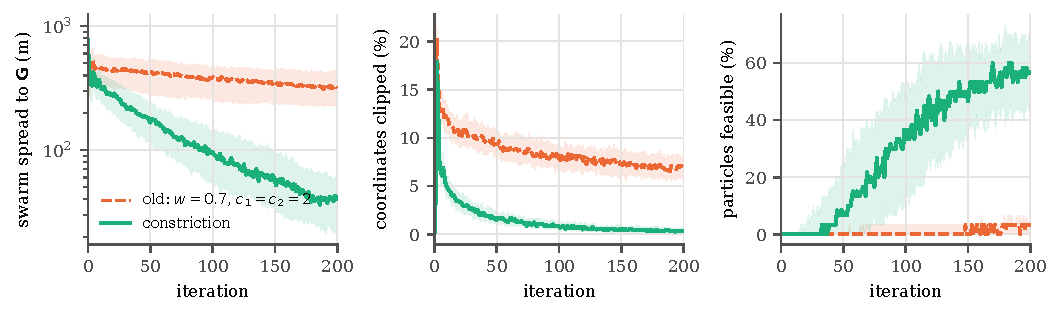
\includegraphics[width=\textwidth]{figures_mpce/diag_pso_dynamics.pdf}
\caption{PSO dynamics with the old setting ($w=0.7$, $c_1=c_2=2$) and the constriction setting on 6 cases $\times$ 10 seeds at 6,030 evaluations (200 iterations): median (line) and interquartile range (band) over the runs. Left: swarm spread, the mean over particles of the RMS distance of the turbines to the global best $\mathbf G$ (log scale). Middle: share of the coordinates that leave the bounding square in an iteration and are clipped (velocities are kept). Right: share of particle evaluations whose layout is feasible. Per-case values: Table~\ref{tab:D-psodyn}.}
\label{fig:D-psodyn}
\end{figure*}

\begin{table*}[!t]
\centering
\caption{PSO dynamics per case, old setting / constriction setting (10 seeds each, 6,030 evaluations). Spread: median over the runs of the swarm spread at the last iteration (m); $|V|$: median mean absolute velocity per coordinate at the last iteration (m); clipped: share of coordinates clipped per iteration (iterations 1--200); feasible, outside, spacing: share of particle evaluations in iterations 101--200 with a feasible layout, with a turbine outside the circle, with two turbines closer than $8R$; $\mathbf G$ feas.: runs whose final global best is feasible; $L$: median wake loss of the feasible final global bests (\%). Note below the table: violations of the infeasible evaluations and of the final layouts of all stored runs of both settings (68 cases $\times$ 30 seeds).}
\label{tab:D-psodyn}
\scriptsize\setlength{\tabcolsep}{3pt}
\begin{tabular}{lcccccccc}
\toprule
Case (DS, $r$, $N$) & Spread (m) & $|V|$ (m) & Clipped (\%) & Feasible (\%) & Outside (\%) & Spacing (\%) & $\mathbf G$ feas. & $L$ (\%) \\
\midrule
I, 500, 6 & 188.9 / 21.7 & 127.7 / 9.5 & 8.8 / 1.9 & 5.8 / 54.8 & 81.0 / 40.6 & 79.3 / 10.6 & 10 / 10 & 0.52 / 0.43 \\
I, 1000, 10 & 436.1 / 58.3 & 268.9 / 21.8 & 8.4 / 1.3 & 3.6 / 66.6 & 87.6 / 23.4 & 85.1 / 17.8 & 10 / 10 & 0.78 / 0.45 \\
I, 750, 12 & 332.1 / 51.4 & 190.5 / 18.6 & 9.1 / 1.6 & 0.7 / 41.9 & 92.9 / 31.1 & 98.8 / 49.0 & 4 / 10 & 3.79 / 1.44 \\
II, 750, 8 & 311.3 / 39.4 & 177.8 / 16.6 & 8.7 / 2.0 & 5.4 / 55.7 & 86.6 / 35.2 & 78.8 / 20.2 & 10 / 10 & 2.67 / 1.82 \\
II, 500, 10 & 197.8 / 14.5 & 125.4 / 4.8 & 8.4 / 1.5 & 0.0 / 27.2 & 89.9 / 36.2 & 100.0 / 64.4 & 0 / 10 & -- / 7.75 \\
II, 1000, 15 & 488.5 / 53.8 & 283.8 / 19.3 & 8.7 / 1.6 & 0.5 / 44.1 & 95.5 / 27.6 & 99.3 / 48.9 & 3 / 10 & 7.13 / 4.94 \\
\midrule
All 6 cases & 319.3 / 40.7 & 187.3 / 15.2 & 8.7 / 1.6 & 2.6 / 48.4 & 88.9 / 32.3 & 90.2 / 35.2 & 37 / 60 & \\
\bottomrule
\end{tabular}
\\[3pt]
\parbox{\textwidth}{\scriptsize Infeasible particle evaluations (iterations 1--200; old / constriction): 98.3 / 68.4\% of all; of these, outside the circle only 5.8 / 18.4\%, spacing only 7.9 / 34.3\%, both 86.3 / 47.3\%. Final layouts of all stored runs (old / constriction; feasibility rule of the paper: a turbine more than $10^{-6}$~m outside the circle, a pair more than $10^{-6}$~m closer than $8R$): infeasible 286 / 0 of 2{,}040; of these, outside the circle only 10 / 0, spacing only 224 / 0, both 52 / 0; with a turbine outside the circle that sits on the box bound at a tangent point ($|x|=r$ or $|y|=r$): 60 / 0. (Spacing from the stored minimum spacing; boundary from the coordinates, which are stored to 1~mm; the 46 old-setting finals whose boundary status is not decidable at 1~mm, or that are among the instrumented runs, are classified with the unrounded positions of the reproduced runs. With a 1-mm tolerance instead, 282 finals are infeasible and 246 violate only the spacing.) Final layouts with a coordinate on the box bound: 68 / 2 (infeasible ones: 60 / 0).}
\end{table*}

\begin{table}[!t]
\centering
\caption{Inside the VNS phase (Phase~2) of the hybrids at 6,030 evaluations: 12 split cases (both data sets; $r=500, 750, 1000$~m with $N=6, 8, 10$ and $N=10, 12, 15$) $\times$ 10 seeds. A cycle is one shaking step followed by the complete local search (compass search); the first descent is the local search from the switch point, before any shaking; every evaluation after it belongs to a cycle. Evaluation shares are pooled over the runs (sum over runs of the evaluations of a stage divided by the sum of the Phase-2 evaluations); medians of the per-run shares are given separately. Improvement shares refer to the reduction of the wake loss in Phase~2 in the runs whose switch point is feasible (pooled); the gain of the cycles includes the local search of a cycle cut off by the budget.}
\label{tab:D-vns}
\scriptsize\setlength{\tabcolsep}{3pt}
\resizebox{\ifdim\width>\columnwidth\columnwidth\else\width\fi}{!}{%
\begin{tabular}{lccc}
\toprule
 & PSO-VNS & SSA-VNS & RS-VNS \\
\midrule
Runs with feasible switch point & 116 of 120 & 100 of 120 & 48 of 120 \\
Phase-2 evaluations (median) & 3{,}000 & 3{,}000 & 3{,}015 \\
First descent: evaluations (median) & 2{,}860 & 2{,}920 & 3{,}015 \\
\quad share of Phase-2 evaluations (pooled, \%) & 78.5 & 75.9 & 84.8 \\
\quad share of Phase-2 evaluations (median over runs, \%) & 95.3 & 97.3 & 100.0 \\
Shake-plus-search cycles: share of Phase-2 evaluations (pooled, \%) & 21.5 & 24.1 & 15.2 \\
\quad in the runs with a feasible switch point (pooled, \%) & 22.3 & 25.8 & 28.1 \\
\quad runs with at least one cycle evaluation & 62 & 62 & 42 \\
Shaking steps per run (median) & 1.0 & 1.0 & 0.0 \\
\quad range over runs & 0--3 & 0--3 & 0--3 \\
\quad median for $N=6$ & 2.0 & 2.0 & 2.0 \\
\quad median for $N=8$ & 1.0 & 1.0 & 1.0 \\
\quad median for $N=10$ & 1.0 & 1.0 & 0.0 \\
\quad median for $N=12$ & 0.0 & 0.0 & 0.0 \\
\quad median for $N=15$ & 0.0 & 0.0 & 0.0 \\
Shaking evaluations (\% of Phase~2; rest: local search) & 0.02 & 0.03 & 0.02 \\
Accepted cycles per run (mean) & 0.1 & 0.1 & 0.1 \\
\quad acceptance rate of cycles (\%) & 22.2 & 25.8 & 80.0 \\
\quad share accepted with $k=1$ (\%) & 100.0 & 100.0 & 100.0 \\
\quad accepted with $k=1,\dots,5$ & 6/0/0/0/0 & 8/0/0/0/0 & 16/0/0/0/0 \\
\quad runs without an accepted cycle & 114 & 112 & 104 \\
\quad shaken point already better (\% of accepted) & 0.0 & 0.0 & 0.0 \\
Improvement from the first descent (pooled, \%) & 97.5 & 90.3 & 88.6 \\
Improvement from accepted cycles (\%) & 0.5 & 3.4 & 3.5 \\
Improvement from all cycles, incl.\ the one cut off (\%) & 2.5 & 9.7 & 11.4 \\
Infeasible at switch, feasible after descent & 1 & 6 & 11 \\
Infeasible at switch, feasible after a cycle & 0 & 0 & 0 \\
Feasible incumbent made infeasible & 0 & 0 & 0 \\
Start is not the best feasible Phase-1 layout$^a$ & 0 & 0 & 0 \\
\bottomrule
\end{tabular}}
\\[2pt]\parbox{\columnwidth}{\scriptsize $^a$ runs in which Phase~1 evaluated at least one feasible layout but handed an infeasible or worse layout to VNS (the penalized comparison picks the best feasible layout whenever one exists).}
\end{table}

\begin{table}[!t]
\centering
\caption{Why PSO (constriction) and DE do not move from feasible starts: the six largest cases and the Horns Rev~1 16-turbine block $\times$ 3 seeds with feasibility-preserving initialization, 6,030 evaluations; every candidate (trial) is logged; feasibility with the 1e-6~m tolerance of the paper. Mixture test: first-update PSO candidates $\mathbf P^i+c_2\,\mathbf r\odot(\mathbf G-\mathbf P^i)$ between a particle's feasible start and the global best (200 draws per particle, separate random stream; $c_2=1.496$, independent $\mathbf r\sim U(0,1)$ per coordinate, clipped to the box), with the original turbine labels and after relabelling the turbines of $\mathbf P^i$ to their nearest turbines of $\mathbf G$ (assignment problem); then, relabelled, without overshoot (weights in $[0,1]$) and with one common weight (a convex combination of the two layouts).}
\label{tab:D-feasstart}
\scriptsize\setlength{\tabcolsep}{3pt}
\resizebox{\ifdim\width>\columnwidth\columnwidth\else\width\fi}{!}{%
\begin{tabular}{lcc}
\toprule
 & PSO & DE \\
\midrule
Runs with an improved global best & 0 of 21 & 0 of 21 \\
Candidates evaluated after the initial population & 126{,}000 & 126{,}000 \\
\quad feasible (\%) & 3.33 & 0.00 \\
\quad feasible, other than re-evaluations of $\mathbf G$ & 0 & 0 \\
Infeasible candidates: outside the site only / spacing only / both (\%) & 0.0 / 3.6 / 96.4 & 0.0 / 0.6 / 99.4 \\
Feasible at the first update (\%) & 3.3 & 0.0 \\
Median min.\ spacing at the first update (m; limit 308, Horns Rev 320) & 95 & 84 \\
Personal-best updates / accepted DE trials & 0 & 0 \\
Feasible candidates better than $\mathbf G$ & 0 & 0 \\
Runs in which the $\mathbf G$-particle keeps $\mathbf V=\mathbf 0$ & 21 of 21 & -- \\
Iterations with exactly one feasible candidate ($\mathbf G$ re-evaluated) & 4{,}200 of 4{,}200 & -- \\
\midrule
\multicolumn{3}{l}{Mixture test (feasible \% / turbine outside the site \% / median min.\ spacing, m):} \\
\quad first PSO move, original labels & \multicolumn{2}{l}{0.0 / 93.1 / 91} \\
\quad first PSO move, relabelled & \multicolumn{2}{l}{0.1 / 80.3 / 189} \\
\quad relabelled, weights in $[0,1]$ & \multicolumn{2}{l}{0.8 / 39.4 / 222} \\
\quad relabelled, one weight (convex comb.) & \multicolumn{2}{l}{16.6 / 0.0 / 286} \\
Initial layouts: RMS turbine distance to $\mathbf G$ after relabelling (m, median / min) & 291 / 111 & \\
\midrule
All stored runs of the paper (30 seeds): final $\ne$ best initial layout & 0 of 210 & 0 of 210 \\
\bottomrule
\end{tabular}}
\end{table}

\begin{table}[!t]
\centering
\caption{Phase~1 of RS-VNS replayed (geometry only, the seeded random stream of the runs): feasible samples among the 3,015 uniform samples in the bounding square, over 30 seeds (90,450 samples per row; the geometry is the same for both data sets). Inside: all $N$ turbines inside the circle, observed rate and $(\pi/4)^N$. Disc: Monte Carlo feasibility rate of the same number of samples uniform in the disc (the Phase-1 distribution of the disc-sampling control RSD-VNS). Rows with $N\le 5$ at 750 and 1000~m omitted (all 30 seeds have feasible samples).}
\label{tab:D-rsreplay}
\scriptsize\setlength{\tabcolsep}{3pt}
\begin{tabular}{rrrrrrr}
\toprule
$r$ (m) & $N$ & feasible & seeds with one & inside (\%) & $(\pi/4)^N$ (\%) & disc feasible (\%) \\
\midrule
500 & 2 & 39{,}952 & 30 & 61.45 & 61.69 & 71.9 \\
500 & 3 & 15{,}525 & 30 & 48.32 & 48.45 & 35.4 \\
500 & 4 & 3{,}740 & 30 & 37.94 & 38.05 & 11.1 \\
500 & 5 & 546 & 30 & 29.76 & 29.88 & 2.11 \\
500 & 6 & 53 & 23 & 23.12 & 23.47 & 0.186 \\
500 & 7 & 1 & 1 & 18.19 & 18.43 & 0.0166 \\
500 & 8 & 0 & 0 & 14.22 & 14.48 & 0 \\
500 & 9 & 0 & 0 & 11.19 & 11.37 & 0 \\
500 & 10 & 0 & 0 & 8.70 & 8.93 & 0 \\
750 & 6 & 1{,}698 & 30 & 23.12 & 23.47 & 8.28 \\
750 & 7 & 458 & 30 & 18.19 & 18.43 & 2.71 \\
750 & 8 & 75 & 25 & 14.22 & 14.48 & 0.711 \\
750 & 9 & 15 & 13 & 11.19 & 11.37 & 0.129 \\
750 & 10 & 2 & 2 & 8.70 & 8.93 & 0.0155 \\
750 & 11 & 0 & 0 & 6.89 & 7.01 & 0.00221 \\
750 & 12 & 0 & 0 & 5.44 & 5.51 & 0 \\
1000 & 6 & 5{,}275 & 30 & 23.12 & 23.47 & 25.1 \\
1000 & 7 & 2{,}264 & 30 & 18.19 & 18.43 & 14.1 \\
1000 & 8 & 906 & 30 & 14.22 & 14.48 & 7.03 \\
1000 & 9 & 280 & 30 & 11.19 & 11.37 & 3.11 \\
1000 & 10 & 101 & 27 & 8.70 & 8.93 & 1.25 \\
1000 & 11 & 23 & 15 & 6.89 & 7.01 & 0.385 \\
1000 & 12 & 8 & 8 & 5.44 & 5.51 & 0.138 \\
1000 & 13 & 1 & 1 & 4.21 & 4.33 & 0.0376 \\
1000 & 14 & 0 & 0 & 3.26 & 3.40 & 0.00663 \\
1000 & 15 & 0 & 0 & 2.64 & 2.67 & 0.00111 \\
\bottomrule
\end{tabular}
\end{table}

